%%
%%                  TEMPLATE for Math 436 project report
%%
\documentclass[11pt]{amsart}
%%% WARNING: Do NOT change the page size, fonts, or margins!  Penalties will apply.


\usepackage{graphicx}
\usepackage{amssymb,amsmath,amsthm}
\usepackage{placeins} %enables \FloatBarrier, which prevents figures and tables from going below it.
\usepackage{hyperref} %makes cross references into hyperlinks. 
 

%%% WARNING: Do NOT change the page size, fonts, or margins!  Penalties will apply.
%%% WARNING: Do NOT change the page size, fonts, or margins!  Penalties will apply.

\begin{document}

\title{Modeling Salvation}
\author{Taylor Rubalcava, Matthew Ward, Matthew  Dangerfield}

% Change the date to match the date you actually wrote this paper
\date{\today} % or use \today

\begin{abstract}
Using key indicator data generated by The Church of Jesus Christ of Latter-Day Saints' missionaries, this paper studies the potential for modeling the growth of church membership in local regions using a variant of a bidirectional SIR model. This model exhibits many of the qualitative behaviors experienced by missionaries on a local scale and is capable of giving reasonable estimates for church membership growth in a local region over the short term. Using this simple model, the potential impacts of changes in the missionary program can be studied and opportunities for potential growth can be found.
\end{abstract}

\maketitle % this actually makes the title

%% First Section
\section{Background/Motivation}

The Church of Jesus Christ of Latter-day Saints has approximately 70,000 missionaries serving in voluntary ecclesiastical service around the world \cite{ChurchNews}. To organize this massive coalition of young adults (usually 18-23 years old) in foreign countries, the Church has a series of \textit{key indicators} that can effectively be thought of as steps in a conversion funnel.

\begin{itemize}
  \item New People (number of individuals beginning to be taught by missionaries)
  \item Sacrament Attendances (number of individuals attending worship services)
  \item People on Date (number of individuals who have scheduled a day to join the church)
  \item Baptisms (number of individuals who have joined the church via baptism)
\end{itemize} \cite{PMG}

These key indicators are used as a metric of success by the missionary department, the missionaries themselves, and represent the experiences of thousands of missionaries and the hundreds of thousands that they teach. A model of the key indicators could be used to explore the impacts of policy change and predict the effects of various situations on Church membership. For example, the Church could have used such a model to predict how changing the age of missionary eligibility or a world-wide pandemic could effect baptisms later on. A mathematical model that can simulate the impacts of these leadership decisions prior to their enactment would be invaluable in avoiding pitfalls and analyzing opportunities for growth. 

We can think of the spread of Church membership as the diffusion of Latter-day Saint faith through a population. For this reason, the SIR model is a strong candidate, since prior work has used SIR-type frameworks to model similar phenomena. Most directly, \cite{hayward1995church} used a SIR model to describe how non-believers become ``infected" through conversion, and then ``infect" their contacts through evangelism. In \cite{koval2023social}, the authors fit a bidirectional three-stage model to 10 years of data on young adult religious participation. We build on this work to create a 5-stage bidirectional model that more specifically models Latter-day Saint church growth.

%% Second Section 
\section{Modeling}

\subsection*{Simplifying Assumptions.}
\begin{center}
\hspace{0pt}
\end{center}

In order to model this complicated system with ODEs, we make the following simplifying assumptions.

\begin{itemize}
    \item All people fall into one of the following ordered categories:
    \begin{enumerate}
        \item Uncontacted
        \item Being taught
        \item Attending Church meetings
        \item On date to join the Church
        \item Church members
    \end{enumerate}
    \item In their progression and regression, people do not skip categories. For example, a person who is uncontacted (1) cannot immediately begin attending Church meetings (3), or vice versa.
    \item Unless otherwise stated below, the rate at which people progress or regress in any category is proportional to the number of people in that category.
    \item Since missionaries have by far the most success when Church members refer their friends for missionary discussions, the rate at which uncontacted people (1) start being taught (2) is also proportional to the number of members of the Church.
    \item We choose not to model those who choose to withdraw from Church membership, so the rate of regression from membership (5) is zero.
\end{itemize}

Note that our 5 stages differ from the traditional Key Indicators used by missionaries. Missionaries use Key Indicators to measure results week-by-week, thus someone could contribute to New Persons and Sacrament Attendances in the same week. In our model, each individual can only be occupy one stage at a time. For example, once someone attends church, they progress from the ``Being taught" stage to the ``Attending Church Meetings" stage.

\begin{samepage}
\subsection*{Constructing the model.}
\begin{center}
\hspace{0pt}
\end{center}

Let $p_i$ with $i \in \{1, ..., 5\}$ represent the proportion of the populations that are uncontacted ($p_1$), being taught ($p_2$), attending sacrament meeting ($p_3$), on date to be baptized ($p_4$), and Church members ($p_5$). These are each functions of time. Together they compose the vector function $\boldsymbol{p}(t) = \left(p_1(t), ..., p_5(t)\right)$.
\end{samepage}

Each $p_i$ has two rates $\alpha_i(t)$ and $\beta_i(t)$ (these may also depend on time) attached to it. $\alpha_i$ is the rate they progress towards joining the Church ($p_i \rightarrow p_{i+1}$), and $\beta_i$ is the rate they regress away from joining the Church ($p_i \rightarrow p_{i-1}$). Hence, setting $p_0$ and $p_6$ (as well as their respective rates $\alpha_0$, $\beta_0$, $\alpha_6$, and $\beta_6$) equal to 0 for ease of notation, letting $t$ represent time, and using Newton's dot-notation for derivatives, for all $i \in \{1, ..., 5\}$ it holds that:

\begin{equation}
\dot{p}_i(t) = \alpha_{i-1}(t) p_{i-1}(t) + \beta_{i+1}(t) p_{i+1}(t) - (\alpha_i(t) + \beta_i(t)) p_i(t)
\label{eq:OrigModel}
\end{equation}

We set $\alpha_5(t) = 0$ since we assume no progression beyond joining the church, we set $\beta_1(t) = 0$ since we assume no regression beyond being uncontacted, and we also set $\beta_5(t) = 0$, since we assume that once a person has joined the church, they do not leave it.

In Equation~\ref{eq:OrigModel}, at the stage of progression $p_i$, $\alpha_{i-1} p_{i-1}$ is the rate at which people progress from the lower stage into stage $p_i$, and $\beta_{i+1} p_{i+1}$ is the rate people regress back to $p_i$ from the next stage along.

The rate at which uncontacted people start being taught is proportional to the number of members, so $\alpha_1(t) = a_1 p_5(t)$ for some constant $a_1$. In this sense, $a_1$ may be thought of as the number of new people being taught per member per unit time. So fix constants $\{a_1, ..., a_4\}$ and $\{b_2, ..., b_4\}$ and define

\begin{equation}
\begin{aligned}
    \alpha_i(t) &= \begin{cases} 
    a_1 p_5(t) & \text{if } i = 1, \\
    a_i & \text{if } i \in \{2, ..., 4\}, \\
    0 & \text{otherwise}
    \end{cases} \\
    \beta_i(t) &= \begin{cases} 
    b_i & \text{if } i \in \{2, ..., 4\}, \\
    0 & \text{otherwise}.
    \end{cases}
\end{aligned}
\label{eq:Rates}
\end{equation}


for all times $t$.

This model is a slight adaptation of the prototypical SIR model, which only allows for forward movement or progression of individuals through states. This model not only allows for backwards movement but it allows for it at every state. 

In summary, combining Equations ~\ref{eq:OrigModel} and ~\ref{eq:Rates}, representing each $p_i(t)$ simply as $p_i$, and representing element-wise multiplication by $\circ$, we have that

\begin{equation}
    \boldsymbol{\dot{p}}
        =
    \begin{pmatrix} \dot{p_1} \\ \dot{p_2} \\ \dot{p_3} \\ \dot{p_4} \\ \dot{p_5} \end{pmatrix}
        =
    \begin{pmatrix} 0 \\ a_1 p_5 \\ a_2 \\ a_3 \\ a_4 \end{pmatrix} 
        \circ 
    \begin{pmatrix} 0 \\ p_1 \\ p_2 \\ p_3 \\ p_4 \end{pmatrix} 
        + 
    \begin{pmatrix} b_2 \\ b_3 \\ b_4 \\ b_5 \\ 0 \end{pmatrix} 
        \circ 
    \begin{pmatrix} p_2 \\ p_3 \\ p_4 \\ p_5 \\ 0 \end{pmatrix} 
        - 
    \left(\begin{pmatrix} a_1 p_5 \\ a_2 \\ a_3 \\ a_4 \\ 0 \end{pmatrix} + \begin{pmatrix} 0 \\ b_2 \\ b_3 \\ b_4 \\ 0 \end{pmatrix}\right) 
        \circ 
    \begin{pmatrix} p_1 \\ p_2 \\ p_3 \\ p_4 \\ p_5 \end{pmatrix}
\label{eq:VectorizedModel}
\end{equation}

\subsection*{Setting Parameters.}
\begin{center}
\hspace{0pt}
\end{center}

\nopagebreak

To show that our model has the behavior we expect, we set the parameters and initial conditions in a reasonable way and observe the results. We let the unit of time be weeks, beginning at $t=0$ so that $\boldsymbol{p}(3)$ represents the state of the system at 3 weeks.

\textit{Initial conditions:}
\begin{itemize}
    \item $p_1 = 0.999$. The vast majority of the population is uncontacted.
    \item $p_2, p_3, p_4 = 0$. Nobody is being taught, attending sacrament meeting, or planning to join the Church.
    \item $p_5 = 0.001$. Church members represent a small proportion of the population.
\end{itemize}

\textit{Parameters:}
\begin{itemize}
    \item $a_1 = \frac{1}{100}$. 1 person begins receiving discussions per 100 Church members per week.
    \item $(a_2, a_3, a_4) = (\frac{1}{3}, \frac{1}{20}, \frac{1}{12})$. Other progress rates (people per week).
    \item $(b_2, b_3, b_4) = (\frac{1}{15}, \frac{1}{2}, \frac{1}{2})$. Rates of regression (people per week).
\end{itemize}

\subsection*{Long-term Simulation.}
\begin{center}
\hspace{0pt}
\end{center}

\nopagebreak

Using the initial conditions and parameters given above, we begin by simulating a long period of time---500 years (see Figure ~\ref{fig:LongTerm}). We see that as Church membership grows, missionary work accelerates, as our assumptions would imply. As Church memberships approaches 100\%, missionary work slows.

While probably unrealistic for any given part of the world (unless the Second Coming happens soon!), this does make sense given the assumptions we have made.

We would like to consider this scenario from the perspective of the missionaries. To do so, we use phase portraits with $p_2$ (the number of people being taught who are not attending Church) at the bottom, since much of a missionary's time is spent looking for and teaching people who are not yet attending Church. For the result, see Figure ~\ref{fig:LongTermPhase}.

\begin{figure}[htb]
\begin{center} %Put your images in a figure like this
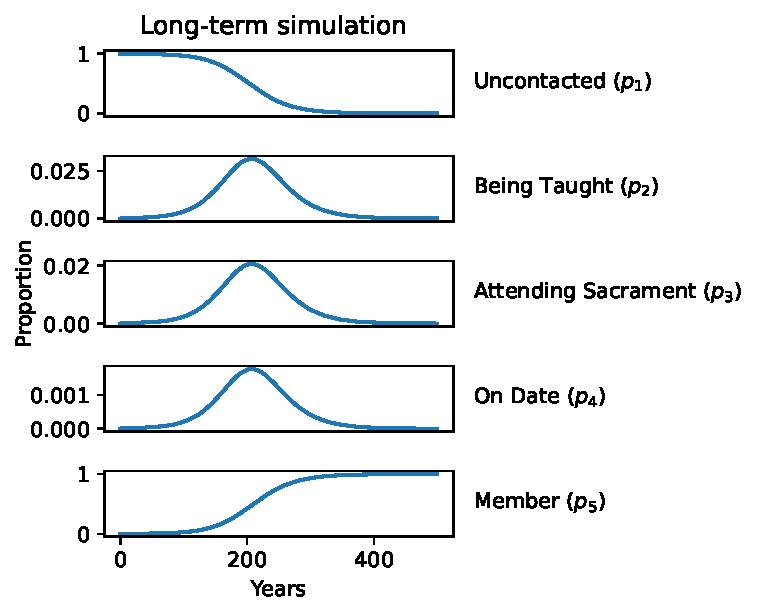
\includegraphics[width=0.7\textwidth]{long-term.pdf}
\end{center}
\caption{500 years of missionary work simulated with plausible initial conditions and parameters. The rate of increase in membership is maximized at around $t = 200$ years.}
\label{fig:LongTerm}
\end{figure}

\begin{figure}[htb]
\begin{center} %Put your images in a figure like this
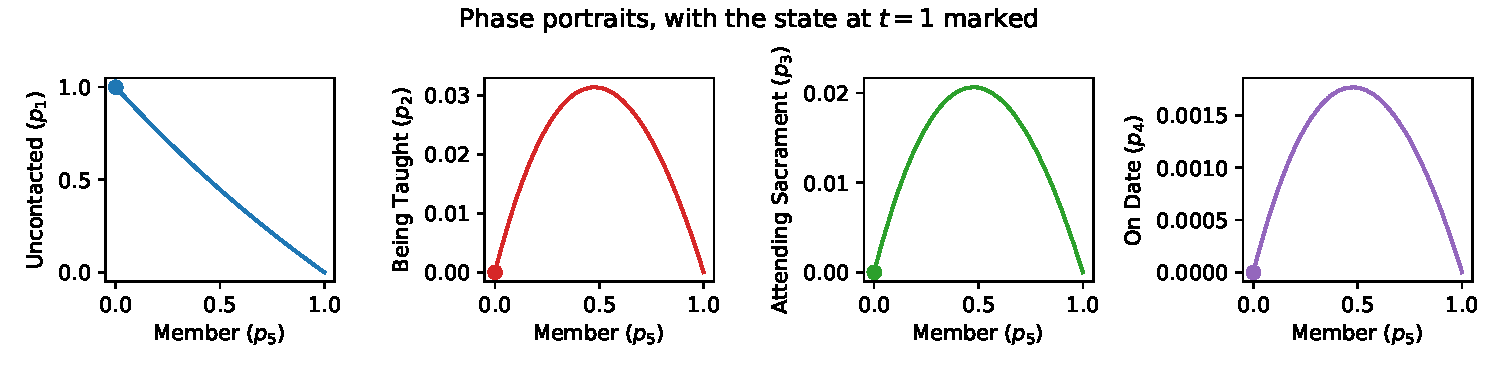
\includegraphics[width=1\textwidth]{long-term-phase.pdf}
\end{center}
\caption{Phase portraits for 500 years of missionary work simulated with plausible initial conditions and parameters (see Figure ~\ref{fig:LongTerm}). In each portrait, we place the number of people being taught on the $x$-axis. We see that when missionaries are "busiest" (teaching the most non-attending people), a bit less than half of the population remains uncontacted, and likewise, a little less than half has joined the Church. The rest are attending Church or on date to join it, with about ten times as many attending as are preparing to join.}
\label{fig:LongTermPhase}
\end{figure}

\begin{samepage}
\subsection*{Data driven short term simulation.}
\begin{center}
\hspace{0pt}
\end{center}

We now test our model's ability to model missionary work in the short term. From weekly data that one of this paper's authors collected from the South American mission in which they served, we inferred values for $\boldsymbol{p}(t)$ at each week over an approximately 2 year period. Using SciPy, we optimized our model's parameters to fit the data. We present the results in Figure ~\ref{fig:ShortTerm}. We list the optimal parameters with brief reminders for what they represent:
\end{samepage}

\begin{samepage}
\begin{itemize}
	\item $a_1 = 0.00030$ (Proportion of new people being taught per member per week)
	\item $a_2 = 0.01883$ (Proportion per week: Being Taught to Attending)
	\item $a_3 = 0.36835$ (Proportion per week: Attending to On Date)
	\item $a_4 = 0.07221$ (Proportion per week: On Date to Member)
	\item $b_2 = 0.90413$ ({Proportion} per week: Being Taught to Uncontacted)
	\item $b_3 = 0.08190$ (Proportion per week: Attending to Being Taught)
	\item $b_4 = 0.45164$ (Proportion per week: On Date to Attending)
\end{itemize}
\end{samepage}

\begin{figure}[htb]
\begin{center} %Put your images in a figure like this
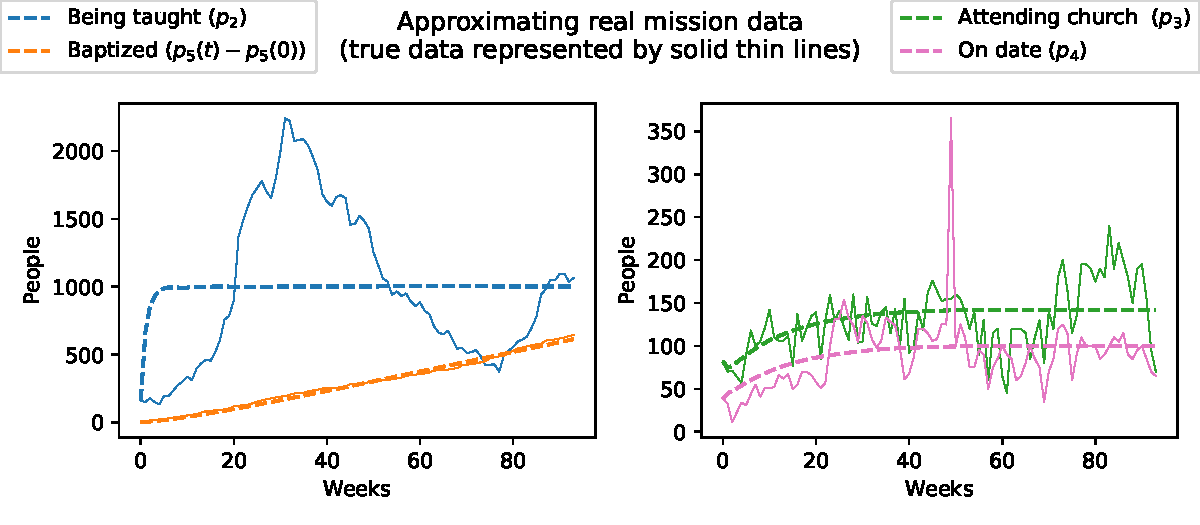
\includegraphics[width=1\textwidth]{fit-data-[[1, 4], [2, 3]].pdf}
\end{center}
\caption{Fitting our model to real data. The model uses proportions internally, but these plots have been rescaled by the population (3 million). In addition, for easy comparison to the number of people being taught ($p_2$), we depict the number of new members (baptisms) since $t=0$ rather than the current number of members. $p_5(0) = 3000$.}
\label{fig:ShortTerm} % for automatic cross referencing
\end{figure}

\begin{samepage}
\subsection*{Model Adaptations.}
\begin{center}
\hspace{0pt}
\end{center}

We also analyzed a couple of alternative models that account for behavior not fully captured by our model. Our current model fails to distinguish between people who have never been contacted by missionaries, and those who have been contacted and have no interest in further contact. A more accurate model would have a sixth category, ``Not Interested", to capture these people. This would mean changing our model as follows:
\end{samepage}

\begin{equation}
\begin{aligned}
\dot{p}_1(t) &= - \alpha_1(t) p_1(t)
\\
\dot{p}_6(t) &= \beta_2(t) p_2(t)
\end{aligned}
\end{equation}

With properly set coefficients, this would lead to everyone eventually being Not Interested, or Baptized.

Another shortcoming of the current model is its unrealistic modeling of the New People rate as being proportional to the number of Baptized members as well as Uncontacted population. Being in a high population area alone doesn't mean that many New People will be taught, especially if the population is significantly larger than the number of church members in the area. Additionally, if an area has a low population, even 1,000 missionaries won't be able to find any more people to teach.

Let $x = \frac{\text{Number of Baptized}}{\text{Number of Uncontacted}}$. We would expect qualitatively different finding rates as $x \to \infty$ (finding is limited only by the number of Uncontacted people) and as $x \to 0$ (finding is limited by the number of missionaries). This motivates the following adjustment to our model:

\begin{equation}
\alpha_1(t) = a_{11} \left(1- \frac{p_5(t)}{p_1(t)}\right) + a_{12}\frac{p_5(t)}{p_1(t)}
\end{equation}

This leads to different finding rates for different types of areas (missionary-limited vs. population-limited). 

%% Third Section
\section{Results}

The model does display many of the quantitative and qualitative behaviors that would be expected from the key indicators. This includes the transient populations (new people, people attending sacrament, and people on date) remaining fairly constant in the short term, reasonable proportions between the various person states, and projecting approximately the same number of individuals attending church, on date to join the church, and being baptized as there actually were. Long term estimates are sensitive to the initial parameters, however. This suggests that the future growth of the Church may be highly sensitive to the world's population growth, the population growth of the Church itself, and numerous other factors that are not accounted for in this model.

When used to model real mission data, as in Figure~\ref{fig:ShortTerm}, we see that because the parameters are fixed, the model cannot capture some aspects of the unpredictability of real-life missionary work in the short term. It can, however, model broader trends.

We concluded that the model could be useful while exploring the potential impacts of policy changes in the short term, but is less reliable due to sensitivity in the parameters for making long-term predictions. 

%%Fourth Section
\section{Analysis/Conclusions}

As stated above, we assert that the adapted SIR model presented here is a reasonable choice for modeling church population in the short term. We see in Figure ~\ref{fig:ShortTerm} that while some of the wild fluctuations in people's progress is not captured, the overall trends for the most part are. The model's shortcomings arise because the data does not perfectly reflect some of the assumptions that the SIR model is based on, namely that individuals move from one state to the next at a rate proportional to their respective populations. The key indicators (specifically new people) do not generally exhibit this behavior, namely with the population of those attending sacrament not increasing at a rate proportional to the population of new people.

We did, however, model church membership in a local area fairly accurately. Just as with virus modeling, and thus from an SIR perspective, this makes sense as we would expect a proselytizing church population to grow at a rate proportional to the number of members. Given the accuracy of the model while predicting church membership, and the original SIR model's ability to predict the evolution of a system, this or a similar model may be capable of predicting the plateau of church membership.


%%%%%%%%%%%%%%%%%%%%%%%%%%%%%%%%%%%%%
%% Bibliography below
%%%%%%%%%%%%%%%%%%%%%%%%%%%%%%%%%%%%%
\FloatBarrier % Keep the figures from being put after the bibliography
\newpage
%% If using bibtex, leave this uncommented
\bibliography{refs} %if using bibtex, call your bibtex file refs.bib
\bibliographystyle{alpha}

%% If not using bibtex, comment out the previous two lines and uncomment those below
% \begin{thebibliography}{99}
% \end{thebibliography}

\end{document}
